\documentclass[12pt]{article}
\usepackage{amsmath}
\usepackage{amsthm}
\usepackage{graphicx,psfrag,epsf}
\usepackage{enumerate}
\usepackage{natbib}
\usepackage{url} % not crucial - just used below for the URL 
\usepackage{algorithm}
\usepackage{algpseudocode}
\usepackage{subfig}
\usepackage{authblk}
\usepackage{verbatim}

%\pdfminorversion=4
% NOTE: To produce blinded version, replace "0" with "1" below.
\newcommand{\blind}{0}

% DON'T change margins - should be 1 inch all around.
\addtolength{\oddsidemargin}{-.5in}%
\addtolength{\evensidemargin}{-.5in}%
\addtolength{\textwidth}{1in}%
\addtolength{\textheight}{-.3in}%
\addtolength{\topmargin}{-.8in}%

%environment
\newtheorem{thm}{Theorem}
\newtheorem{lem}{Lemma}
\newtheorem{cor}{Corollary}
\newtheorem{prop}{Proposition}
\newtheorem*{defi*}{Properties}
\newtheorem{asn}{Assumption}
\newcommand*\mean[1]{\bar{#1}}
%\newproof{proof}{Proof}
%\newproof{proof}{Proof}
\begin{document}

\def\spacingset#1{\renewcommand{\baselinestretch}%
{#1}\small\normalsize} \spacingset{1}

\title{\bf Appendix of Local Distance Correlation}
\author[1]{Cencheng Shen\thanks{cshen@temple.edu}}
\author[2]{Joshua T. Vogelstein\thanks{jovo@jhu.edu}}
\author[3]{Carey E. Priebe\thanks{cep@jhu.edu}}
\affil[1]{Department of Statistics, Temple University}
\affil[2]{Department of Biomedical Engineering and Institute of Computational Medicine, Johns Hopkins University}
\affil[3]{Department of Applied Mathematics and Statistics, Johns Hopkins University}
\maketitle

\newpage
\spacingset{1.45} % DON'T change the spacing!

%tba: re-organize propositions in appendix and paper?
\section{Proofs}
\begin{thm}
\label{thm1}
Local distance correlation is consistent for testing independence against all alternatives, i.e., the testing power $\beta \rightarrow 1$ as $n \rightarrow \infty$. 
\end{thm}
\begin{proof}
The power of local distance correlation satisfies
\begin{equation}
\beta=\max_{k,l}\{\beta(dCorr_{kl}), k,l\in [2,\ldots,n]\} \geq \beta(dCorr_{n}).
\end{equation}

When testing independence against any alternative, as $n \rightarrow \infty$ we have $\beta(dCorr_{n}) \rightarrow 1$ by \cite{SzekelyRizzoBakirov2007}. It follows that $\beta \rightarrow 1$, and local distance correlation is also consistent.

Note that local modified distance correlation $\{mdCorr_{kl}\}$ is also consistent, by the consistency of global modified distance correlation in \cite{SzekelyRizzo2013a}.
\end{proof}

Next we prove a number of useful propositions for local distance correlation. In particular, proposition 1-4 indicate that one should fix neighborhood ratio $(\frac{k}{n},\frac{l}{n})$ rather than neighborhood size $(k,l)$ when determining the optimal neighborhood.
\begin{prop}
\label{prop1}
1. For any $k,l$ we have
\begin{align*}
dVar_{k}(\mathcal{X}) &= O(p), \\
dVar_{l}(\mathcal{Y}) &= O(q), \\
dCov_{kl}(\mathcal{X},\mathcal{Y}) &= O(\min\{p,q\}), \\
|dCorr_{kl}(\mathcal{X},\mathcal{Y})| &\leq 1, 
\end{align*}
where $p=\frac{k}{n}$ and $q=\frac{l}{n}$. 

2.
For any fixed $(p,q)$ with $k=pn, l=qn$, we have as $n \rightarrow \infty$, 
\begin{align*}
dCov_{kl}(\mathcal{X},\mathcal{Y}) & \rightarrow E(dCov_{kl}(\mathcal{X},\mathcal{Y})) = E(A^{H}_{ij}B^{H}_{ij}I(A_{ij}< \epsilon_{A_{j}})I(B_{ij}< \epsilon_{B_{j}})), \\
dVar_{k}(\mathcal{X}) & \rightarrow E(dVar_{k}(\mathcal{X}))=E(A^{H}_{ij}A^{H}_{ij}I(A_{ij}< \epsilon_{A_{j}})), \\
dVar_{l}(\mathcal{Y}) & \rightarrow E(dVar_{l}(\mathcal{Y}))=E(B^{H}_{ij}B^{H}_{ij}I(B_{ij}< \epsilon_{B_{j}})),
\end{align*}
where $\epsilon_{A_{j}}$ and $\epsilon_{B_{j}}$ are two random variables satisfying $Prob(A_{ij}< \epsilon_{A_{j}} | X_{j})=p$ and $Prob(B_{ij}< \epsilon_{B_{j}} | Y_{j})=q$.

3. For any $k,l$, we have 
\begin{align*}
dVar_{k}(\mathcal{X})=0 &\Leftrightarrow X \mbox{ is degenerate}, \\
dVar_{l}(\mathcal{Y})=0 &\Leftrightarrow Y \mbox{ is degenerate}. 
\end{align*}

When neither $X$ nor $Y$ is degenerate, we further have 
\begin{align*}
dVar_{k}(\mathcal{X}) \rightarrow 0 &\Leftrightarrow p \rightarrow 0, \\
dVar_{l}(\mathcal{Y}) \rightarrow 0 &\Leftrightarrow q \rightarrow 0, \\
dCov_{kl}(\mathcal{X},\mathcal{Y}) \rightarrow 0 &\Leftrightarrow \min\{p,q\} \rightarrow 0.
\end{align*}

4. Suppose $X$ and $Y$ are non-degenerate, and neither $p$ nor $q$ converges to $0$. Then we have
\begin{align*}
dCorr_{kl}(\mathcal{X},\mathcal{Y}) & \rightarrow \frac{E(dCov_{kl}(\mathcal{X},\mathcal{Y}))}{\sqrt{E(dVar_{k}(\mathcal{X}))E(dVar_{l}(\mathcal{Y}))}}\\
&=\frac{E(A^{H}_{ij}B^{H}_{ij}I(A_{ij}< \epsilon_{A_{j}})I(B_{ij}< \epsilon_{B_{j}}))}{\sqrt{E(A^{H}_{ij}A^{H}_{ij}I(A_{ij}< \epsilon_{A_{j}}))E(B^{H}_{ij}B^{H}_{ij}I(B_{ij}< \epsilon_{B_{j}})})}. 
\end{align*}

5. Suppose $X$ and $Y$ are non-degenerate. Then under the null hypothesis that $X$ is independent of $Y$, we have
\begin{align*}
E(dCov_{kl}(\mathcal{X},\mathcal{Y})) \geq 0,
\end{align*}
with equality holds if and only if $\max\{p,q\} = 1$. 

It follows that $dCov_{kl}$ and $dCorr_{kl}$ are asymptotically no less than $0$ for any $k,l$.

6. In the permutation test, the power of local distance covariance is the same as the power of local distance correlation, because $\beta(dCorr_{kl})=\beta(dCov_{kl})$ for all $k,l$. The p-value of local distance covariance is also the same as that of local distance correlation.
\end{prop}
\begin{proof}
1.

For local distance covariance, we have
\begin{align*}
|dCov_{kl}(\mathcal{X},\mathcal{Y})| &= \frac{1}{n^2} |\sum_{i,j=1}^{n}A^{H}_{ij}B^{H}_{ij}I(r(A_{ij})<k)I(r(B_{ij})<l) | \\
                                   & \leq \frac{1}{n^2} \max_{i,j}|A^{H}_{ij}B^{H}_{ij}| \cdot \min\{kn,ln\} \\
																	 & = O(\min\{p,q\}),
\end{align*}
where the last equality follows from the finite second moments assumption such that $A^{H}_{ij}B^{H}_{ij}$ is bounded. Similarly we can derive that $dVar_{k}(\mathcal{X}) = O(p)$ and $dVar_{l}(\mathcal{Y}) = O(q)$. 

Since $|dCov_{kl}| \leq \sqrt{dVar_{k} \cdot dVar_{l}}$ by the Cauchy-Schwartz inequality, we immediately have $|dCorr_{kl}| \leq 1$ for any $k,l$.

2.

For each $i,j$, $A_{ij}=\|X_{i}-X_{j}\|_{2}$ such that $A_{ij}$ is only correlated with $A_{is}, A_{si},A_{js}, A_{sj}$ for $s=1,\ldots,n$. Thus there are at most $4n$ out of $n^2$ distance entries in $A$ that are correlated with each $A_{ij}$.

Since $A^{H}=HAH$, we have 
\begin{align*}
A^{H}_{ij}=A_{ij}-\bar{A_{i\cdot}}-\bar{A_{\cdot j}}+\bar{A_{\cdot \cdot}},
\end{align*}
where $\bar{A_{i\cdot}}=\sum_{s=1}^{n}\frac{A_{is}}{n}$, $\bar{A_{\cdot j}}=\sum_{s=1}^{n}\frac{A_{sj}}{n}$, and $\bar{A_{\cdot \cdot}}=\sum_{s,t=1}^{n}\frac{A_{st}}{n^2}$. Thus for each $A^{H}_{ij}$, it is correlated with all of $A^{H}_{st}$ at least through the centering terms.

But when $i, j \notin \{s, t\}$, we have
\begin{align*}
Cov(A_{ij}, A^{H}_{st}) &= Cov(A_{ij},A_{st}-\bar{A_{s\cdot}}-\bar{A_{\cdot t}}+\bar{A_{\cdot \cdot}}) \\
&=Cov(A_{ij},-\frac{A_{si}+A_{sj}}{n}-\frac{A_{it}+A_{jt}}{n}+2\sum_{s=1}^{n}\frac{A_{is}+A_{sj}}{n^2}) \\
&=O(\frac{Var(A_{ij})}{n}) \\
&= O(\frac{1}{n}),
\end{align*}
where the last equality follows from the finite second moments of $X$ such that $Var(A_{ij})$ is bounded above. Similarly we have 
\begin{align*}
Cov(A_{ij}I_{ij}, A^{H}_{st}I_{st}) &= Cov(A_{ij}I_{ij},A_{st}I_{st}-\bar{A_{s\cdot}}I_{st}-\bar{A_{\cdot t}}I_{st}+\bar{A_{\cdot \cdot}}I_{st}) \\
&=Cov(A_{ij}I_{ij},A_{st}I_{st}) + Cov(A_{ij}I_{ij},-\frac{A_{si}+A_{sj}}{n}I_{st} \\
&-\frac{A_{it}+A_{jt}}{n}I_{st}+2\sum_{s=1}^{n}\frac{A_{is}+A_{sj}}{n^2}I_{st}) \\
&=Cov(A_{ij}I_{ij},A_{st}I_{st}) + O(\frac{1}{n}) \\
& \rightarrow O(\frac{1}{n}),
\end{align*}
where we simplify $I(r(A_{ij})<k)$ to $I_{ij}$ and $I(r(A_{st})<k)$ to $I_{st}$. Note that $Cov(A_{ij}I_{ij},A_{st}I_{st}) \rightarrow 0$: when $i, j \notin \{s, t\}$, $A_{ij}$ and $A_{st}$ are independent, while $I_{ij}$ and $I_{st}$ are asymptotically independent. The latter follows from the fact that $I(r(A_{ij})<k) \rightarrow I(A_{ij} < \epsilon_{A_{j}})$, where $\epsilon_{A_{j}}$ satisfies $\int_{0}^{\epsilon_{A_{j}}}A_{ij}dA_{ij} | X_{j}= \frac{k}{n}=p$ and is thus independent from $\epsilon_{A_{t}}$ for given $p$. 

It is similar to see that when $i, j \neq s, t$, we have 
\begin{align*}
&Cov(A^{H}_{ij}A^{H}_{ij}, A^{H}_{st}A^{H}_{st}) =O(\frac{1}{n}) \\
&Cov(A^{H}_{ij}A^{H}_{ij}I(r(A_{ij})<k), A^{H}_{st}A^{H}_{st}I(r(A_{st})<k)) \rightarrow O(\frac{1}{n}). 
\end{align*}
When either $i$ or $j$ takes value in $\{s,t\}$, the covariance is always of $O(1)$. It follows that the variance of $dVar_{k}(\mathcal{X})$ is asymptotically $O(\frac{1}{n})$, such that 
\begin{align*}
dVar_{k}(\mathcal{X}) &\rightarrow E(dVar_{k}(\mathcal{X}))=E(A^{H}_{ij}A^{H}_{ij}I(A_{ij}< \epsilon_{A_{j}}))
\end{align*}
by the weak law of large numbers.

The convergence proof is similar for $dVar_{k}(\mathcal{Y})$ and $dCov_{kl}(\mathcal{X},\mathcal{Y})$. 

3. 

If $X$ is degenerate, i.e., $X$ is almost surely a constant, then clearly $A_{ij}=0$ for all $i,j$ such that $A^{H}_{ij}=0$, and $dVar_{k}(\mathcal{X})=0$ for any $k=1,\ldots,n$.

Suppose for some $k$ such that $dVar_{k}(\mathcal{X})=0$, then we must have $A_{ii}^{H}=0$ for all $i$, i.e., $\bar{A_{\cdot \cdot}}=2\bar{A_{i\cdot}}$ for all $i$. Since $\sum_{i=1}^{n} \bar{A_{i\cdot}}=n\bar{A_{\cdot \cdot}}$, it follows that $\bar{A_{i\cdot}}=0$ for all $i$. Thus $A_{ij}=0$ for all $i,j$, such that $X$ is degenerate.

The same holds for $dVar_{l}(\mathcal{Y})$ such that it is $0$ if and only if $Y$ is degenerate.

When $X$ is non-degenerate, $dVar_{k}(\mathcal{X}) > 0$ always holds. However, as $dVar_{k}(\mathcal{X}) = O(p)$, $dVar_{k}(\mathcal{X}) \rightarrow 0$ if and only if $p \rightarrow 0$. A similar argument works for $dVar_{l}(\mathcal{Y})$ and $dCov_{kl}(\mathcal{X},\mathcal{Y})$.

4. 

When $X$ and $Y$ are non-degenerate, both distance variances are always positive by Proposition 3). It immediately follows that  
\begin{align*}
dCorr_{kl}(\mathcal{X},\mathcal{Y}) & \rightarrow \frac{E(A^{H}_{ij}B^{H}_{ij}I(A_{ij}< \epsilon_{A_{j}})I(B_{ij}< \epsilon_{B_{j}}))}{\sqrt{E(A^{H}_{ij}A^{H}_{ij}I(A_{ij}< \epsilon_{A_{j}}))E(B^{H}_{ij}B^{H}_{ij}I(B_{ij}< \epsilon_{B_{j}})})}. 
\end{align*}
when neither $p$ nor $q$ converges to $0$.

5. 
At $l=n$, it follows that
\begin{align*}
E(dCov_{kn}(\mathcal{X},\mathcal{Y})) &=E(A^{H}_{ij}B^{H}_{ij}I(A_{ij}< \epsilon_{A_{j}})) \\
&=E(A^{H}_{ij}I(A_{ij}< \epsilon_{A_{j}}))E(B^{H}_{ij}) \\
&=0 
\end{align*}
for any $k=1,\ldots,n$, because $E(B^{H}_{ij})=0$ and $A$ is independent of $B$ under the null hypothesis. Similarly $E(dCov_{nl}(\mathcal{X},\mathcal{Y}))=0$ for any $l=1,\ldots,n$.

When $k,l \neq n$, we have 
\begin{align*}
E(dCov_{kl}(\mathcal{X},\mathcal{Y})) &= E(A^{H}_{ij}B^{H}_{ij}I(A_{ij}< \epsilon_{A_{j}})I(B_{ij}< \epsilon_{B_{j}})) \\
&=E(A^{H}_{ij}B^{H}_{ij}I(A_{ij}< \epsilon_{A_{j}}))-E(A^{H}_{ij}B^{H}_{ij}I(A_{ij}< \epsilon_{A_{j}})I(B_{ij} \geq \epsilon_{B_{j}})) \\
&=-E(A^{H}_{ij}I(A_{ij}< \epsilon_{A_{j}}))E(B^{H}_{ij}I(B_{ij} \geq \epsilon_{B_{j}})) \\
&> 0.
\end{align*}
The last inequality follows because $E(A^{H}_{ij}I(A_{ij}< \epsilon_{A_{j}})) \leq 0$ with equality holds if $X$ is degenerate or $p=1$ (i.e.,$\int_{0}^{\epsilon_{A_{j}}}A_{ij} | X_{j}=1$ for all $X_{j}$ in the support of $X$), by the fact that 
\begin{align*}
E(A^{H}_{ij})=E(A^{H}_{ij}I(A_{ij}< \epsilon_{A_{j}})) &+ E(A^{H}_{ij}I(A_{ij}\geq \epsilon_{A_{j}}))=0,\\
E(A^{H}_{ij}I(A_{ij}< \epsilon_{A_{j}})) &\leq E(A^{H}_{ij}I(A_{ij}\geq \epsilon_{A_{j}}));
\end{align*} 
and similarly $E(B^{H}_{ij}I(B_{ij} \geq \epsilon_{B_{j}})) \geq 0$ with equality holds if $Y$ is degenerate or $q=1$.

Then by Proposition 2) and 4), $dCov_{kl}$ and $dCorr_{kl}$ are asymptotically no less than $0$ under the null hypothesis.

6. In the permutation test, the p-value of $dCorr_{kl}$ for given $k,l$ is derived by comparing $dCorr_{kl}(\mathcal{X},\mathcal{Y})$ to $\{dCorr_{kl}(\mathcal{X},\mathcal{Y}P)\}$ containing all permutation matrices $P$. 

Since $dVar_{kl}(\mathcal{Y}P)=dVar_{kl}(\mathcal{Y})$ for any permutation matrix $P$, the p-value is the same by comparing $dCov_{kl}(\mathcal{X},\mathcal{Y})$ to $\{dCov_{kl}(\mathcal{X},\mathcal{Y}P)\}$. 

So the p-values are always the same between local distance covariance and local distance correlation; and it follows that the permutation test powers are also the same.
\end{proof}

%\begin{lem}
%\label{lem2}
%For the permutation test, the p-value of $dCorr_{k}$ is the same as the p-value of $dCov_{k}$ for each $k=1,\ldots,n$.

%For the independence test against fixed marginals, the asymptotic testing power of $dCorr_{k}$ is the same as the asymptotic power of $dCov_{k}$, for any $k$ such that $E(dVar_{k}(\mathcal{X}))$ and $E(dVar_{k}(\mathcal{Y}))$ are non-zero.
%\end{lem}
%\begin{proof}
%In case of permutation test, we are comparing $dCorr_{k}(\mathcal{X},\mathcal{Y})$ and $dCorr_{k}(\mathcal{X},\mathcal{Y}P)$ for random permutation matrices $P$. Since $dVar_{k}(\mathcal{Y})=dVar_{k}(\mathcal{Y}P)$ for any permutation matrix $P$, clearly $dCorr_{k}$ is always equivalent to $dCov_{k}$ in the permutation test.

%In case of the independence test against fixed marginals, $E(dVar_{k}(\mathcal{X}))$ under the null and the alternative has the same value, so is $E(dVar_{k}(\mathcal{Y}))$. When neither expectation is $0$, $dCorr_{k}$ is approximately a scalar multiple of $dCov_{k}$ for large $n$, so their testing power is asymptotically the same.
%\end{proof}

\begin{thm}
\label{thm2}
Suppose $Y=cX$ for a non-zero scalar $c$, then for any $n$ we always have
\begin{equation}
\label{equ1}
\beta(dCorr_{n}) \geq \beta(dCorr_{kl})
\end{equation}
for all $k,l=2,\ldots,n$, where $\beta$ is the permutation test power at a given type $1$ error $\alpha$.

Thus local distance correlation is no better than global distance correlation under linear dependency.
\end{thm}
\begin{proof}
Let us first suppose no two columns of $\mathcal{X}$ have the same magnitude, which holds with probability $1$ if $X$ is continuously distributed. 

Then under linear dependency, it is clearly the case that 
\begin{equation}
\label{cond1}
dCov_{n}(\mathcal{X}, \mathcal{Y}) = c \cdot dVar_{n}(\mathcal{X}) \geq dCov_{n}(\mathcal{X}, \mathcal{Y}P)
\end{equation}
for all possible permutations $P$. The equality holds if and only if $P$ is the identity permutation, such that the p-value of $dCov_{n}$ is always $\frac{1}{n!}$. 

Since $dCov_{kl}(\mathcal{X}, \mathcal{Y})=dCov_{kl}(\mathcal{X}, \mathcal{Y}I)$ for the identity permutation as well, the p-value of $dCov_{kl}$ is at least $\frac{1}{n!}$; thus the p-value of $dCov_{kl}$ is larger than or equal to the p-value of $dCov_{n}$ for all $(k,l) \neq (n,n)$. 

The above result still holds if some or all sample points in $\mathcal{X}$ have the same magnitude. For example, if two columns of $\mathcal{X}$ coincide with each other, Equation~\ref{cond1} still holds for all permutation matrices, but the equality holds when $P$ is either identity or permutes only the same two columns; it follows that the p-value of $dCov_{n}$ becomes $\frac{2}{n!}$, which is still no larger than the p-value of $dCov_{kl}$ for any $(k,l) \neq (n,n)$ by the same argument in the previous paragraph. A similar argument shows that the p-value of $dCov_{n}$ is always the smallest when there are more than two sample points that coincide with each other.

Thus for any given sample data, the p-value of $dCov_{kl}$ is always larger than or equal to the p-value of $dCov_{n}$. Then at any given type $1$ error level $\alpha$, either the alternative hypothesis is rejected by both test statistics when both p-values are higher than $\alpha$, or it is always accepted when both p-values are lower than $\alpha$, or it is accepted only by $dCov_{n}$ when only the p-value of $dCov_{n}$ is lower than $\alpha$. Thus at any given $\alpha$, we must have $\beta(dCov_{n}) \geq \beta(dCov_{kl})$ for all $(k,l) \neq (n,n)$.

By Proposition 6) on the equivalence of local distance covariance and local distance correlation in the permutation test, it follows that Equation~\ref{equ1} holds. So global distance correlation $dCorr_{n}$ cannot be worse than local distance correlation $\{dCorr_{kl}\}$ under linear dependency.
\end{proof}

\begin{thm}
\label{thm3}
There exists $f_{XY}$, $n$ and $\alpha$ such that 
\begin{equation}
\label{equ2}
\beta(dCorr_{n}) > \beta(dCorr_{kl})
\end{equation}
for some $(k,l) \neq (n,n)$, where $\beta$ is the permutation test power at the type $1$ error $\alpha$.

Thus local distance correlation can be better than global distance correlation under certain nonlinear dependency.
\end{thm}
\begin{proof}
We give a simple discrete example of $f_{XY}$ at $n=6$ such that the p-value of $dCov_{kl}$ for $(k,l) \neq (n,n)$ is always lower than the p-value of $dCov_{n}$, which is equivalent to say the permutation test power $\beta(dCov_{n})$ is smaller than $\beta(dCov_{kl})$ at an appropriate type $1$ error level $\alpha$.

Suppose under the alternative, $f_{XY}$ is distributed as follows:
\begin{align*} 
X &\in \{-1,-0.6,-0.2,0.2,0.6,1\} \mbox{ without replacement}, \\
Y &= X^2,
\end{align*}
which is a discrete version of the quadratic relationship in the simulations.

In this example we can easily consider all possibilities of $A^{H}_{ij}$ and $B^{H}_{ij}$, and calculate $dCov_{kl}(\mathcal{X}, \mathcal{Y})$ and $\{dCov_{kl}(\mathcal{X}, \mathcal{Y}P)\}$ for all $k,l=2,\ldots,6$ and all permutation matrices. For example, $dCov_{6}(\mathcal{X}, \mathcal{Y})=\frac{128}{75}$, $dCov_{26}(\mathcal{X}, \mathcal{Y})=\frac{399}{212}$, and similarly all possible permuted test statistics. It follows that the p-value of $dCov_{26}$ is $\frac{4}{15}$, while the p-value of $dCov_{6}$ is $\frac{53}{90}$. 

Note that although the p-value of $dCov_{kl}$ is less than $dCov_{n}$ in the above example, neither p-value are very significant. In fact, we can always consider equally spaced sample points in $[-1,1]$ for $X$, increase $n$ and reach the same conclusion with smaller p-values. Say at $n=9$, the p-value of $dCov_{29}$ is $0.056$ while the p-value of $dCov_{9}$ is $0.4264$. But the computation of all possible permuted test statistics becomes much more time-consuming as $n$ increases, and only approximate p-values can be derived with random permutations for larger $n$.

Therefore we have an example of $f_{XY}$ and $n$ such that $\beta(dCov_{n}) < \beta(dCov_{kl})$ for some $(k,l) \neq (n,n)$: by choosing $\alpha=0.3$, at $n=6$ we have $0=\beta(dCov_{6}) < \beta(dCov_{26})=1$; by choosing $\alpha=0.06$, at $n=9$ we have $0=\beta(dCov_{9}) < \beta(dCov_{29})=1$; 

It follows that Equation~\ref{equ2} holds by Proposition 6), since local distance correlation is equivalent to local distance covariance in the permutation test. Thus local distance correlation $\{dCorr_{kl}\}$ can be better than the global distance correlation $dCorr_{n}$ under certain nonlinear dependency. 
\end{proof}

\section{Simulations Set-Up}
Here we list the exact dependencies for the $20$ types of distributions used in the simulation section of the main paper. In the following, type 1-9 are based on the same function types from \cite{SimonTibshirani2012}, with slightly different coefficients for some and an additional exponential dependency; type 10 corresponds to the uncorrelated binomial example on the Wikipedia page of uncorrelated random variable\footnote{\url{https://en.wikipedia.org/wiki/Uncorrelated_random_variables}}; type 11-17 are exactly the same simulations used by \cite{GorfineHellerHeller2012}, which also appears on the Wikipedia page of correlation\footnote{\url{https://en.wikipedia.org/wiki/Correlation_and_dependence}}; type 18-20 are from the distributions used in \cite{SzekelyRizzoBakirov2007}.

As a reminder, we have $\mathcal{X}=[X_{1},\cdots, X_{n}] \in \mathcal{R}^{m_{X} \times n}$ and $\mathcal{Y}=[Y_{1},\cdots, Y_{n}] \in \mathcal{R}^{m_{Y} \times n}$ with $(X_{i}, Y_{i}) \stackrel{i.i.d.}{\sim} f_{XY}$, where $n$ is the sample size and $m_{X}$ and $m_{Y}$ are the dimensions. We considered two scenarios, a dimension $1$ scenario and an increasing dimension scenario. For the dimension $1$ scenario we always have $m_{X}=m_{Y}=1$, while in the increasing dimension scenario we let $m_{X}$ increase, with $m_{Y}=1$ for type $1-16$ and $m_{Y}=m_{X}$ for type $17-20$. 

For the purpose of increasing dimension scenario, we denote $A$ as a size $1 \times m_{X}$ vector with $A_{i}=\frac{1}{i}$. Thus $AX$ is a dimension $1$ random variable that is a decaying weighted summation of $X$, which equals $X$ when $m_{X}=1$.
 
The noiseless distribution for each type is listed below, where we may use $Z, U, V, Q$ to denote some auxiliary random variables.

1. Linear: $X \sim Uniform(-1,1)^{m_{X}}$, $Y=AX$. 

2. Quadratic: $X \sim Uniform(-1,1)^{m_{X}}$, $Y=(AX)^2$.

3. Cubic: $X \sim Uniform(-1,1)^{m_{X}}$, $Y=128(AX-\frac{1}{3})^3+48(AX-\frac{1}{3})^2-12(AX-\frac{1}{3})$.

4. Sine Period 1/2: $X \sim Uniform(-1,1)^{m_{X}}$, $Y=sin(4\pi \frac{AX}{\max(AX)})$.

5. Sine Period 1/8: $X \sim Uniform(-1,1)^{m_{X}}$, $Y=sin(16\pi \frac{AX}{\max(AX)})$.    

6. $X^\frac{1}{4}$: $X \sim Uniform(-1,1)^{m_{X}}$, $Y=|AX|^\frac{1}{4}$.

7. Circle: $X \sim Uniform(-1,1)^{m_{X}}$, $Z \sim Bernoulli(0.5)$, $Y=(2Z-1) \cdot |1-(2\frac{AX}{\max(AX)}-1)^2|^{\frac{1}{2}}$.

8. Step function: $X \sim Uniform(-1,1)^{m_{X}}$, $Y=I(AX>E(AX))$, where $E(AX)$ is the mean of $AX$ and $I$ is the indicator function. Note that in the simulation code the sample mean is used instead.

9. Exp(X): $X \sim Uniform(-1,1)^{m_{X}}$, $Y=exp(AX)$.

10. Uncorrelated Binomial: $X \sim Bernoulli(0.5)^{m_{X}}$, $Z \sim Bernoulli(0.5)^{m_{X}}$, $Y=AX \cdot A(2Z-1)$.

11. W: $X \sim Uniform(-1,1)^{m_{X}}$, $Z \sim Uniform(-1,1)^{m_{X}}$, $Y=4( ( (AX)^2 - \frac{1}{2} )^2 + AZ/500 )$.

12. Square: Let $U \sim Uniform(-1,1)^{m_{X}}$, $V \sim Uniform(-1,1)^{m_{X}}$, $\theta=-\frac{\pi}{8}$. Then $X=AU \cos(\theta) + AV \sin(\theta), Y=-AU \sin(\theta) + AV \cos(\theta)$.

13. Diamond: Let $U \sim Uniform(-1,1)^{m_{X}}$, $V \sim Uniform(-1,1)^{m_{X}}$, $\theta=-\frac{\pi}{4}$. Then $X=AU \cos(\theta) + AV \sin(\theta), Y=-AU \sin(\theta) + AV \cos(\theta)$.

14. Parabola: $X \sim Uniform(-1,1)^{m_{X}}$, $Q \sim Uniform(0,1)$, $Y=( (AX)^2  + Q)/2$. Note that this is like a noisy version of type 2 quadratic.

15. Two Parabolas: $X \sim Uniform(-1,1)^{m_{X}}$, $Q \sim Uniform(0,1)$, $Z \sim Bernoulli(0.5)$, $Y=( (AX)^2  + Q) \cdot (Z-\frac{1}{2})$.

16. Circle 2: Let $U \sim Uniform(-1,1)^{m_{X}}$, $Q \sim Normal(0,1)$, $Z \sim Normal(0,1)$. Then $X=\sin(AU \pi)+\frac{Q}{8}$, $Y=\cos(AU \pi)+\frac{Q}{8}$. Note that this is a different circle distribution from type 7: it is constructed based on trigonometry and already includes certain noise; although at dimension $1$ they are quite similar, their dependencies in increasing dimension are of larger discrepancy.

17. Independent Clouds: Let $U \sim Normal(0,1)^{m_{X}}$, $V \sim Normal(0,1)^{m_{Y}}$, $Z \sim Bernoulli(0.5)$, $Q \sim Bernoulli(0.5)$. Then we set $m_{X}=m_{Y}$, and take $X=AU/3+Z, Y=AV/3+Q$.

18. Joint Normal: Set $m_{X}=m_{Y}$. Denote $\rho=\frac{1}{2m_{X}}$, $I_{m_{X}}$ as the identity matrix of size $m_{X} \times m_{X}$, $J_{m_{X}}$ as the matrix of ones of size $m_{X} \times m_{X}$, and $\Sigma = \begin{bmatrix} I_{m_{X}}&\rho J_{m_{X}}\\ \rho J_{m_{X}}&I_{m_{X}} \end{bmatrix}$. Then let $(X,Y) \sim Normal(0, \Sigma)$.

19. $Log(X^2)$: $X \sim Normal(0, 1)^{m_{X}}$, $Y=log(X^2)$.

20. Multiplicative Noise: $X \sim Normal(0, 1)^{m_{X}}$, $Z \sim Normal(0, 1)$, $Y=X \cdot Z$.

For each distribution, $X$ and $Y$ are dependent under the alternative (except type 17). By generating the sample data and calculating the sample test statistic for sufficiently many Monte-Carlo replicates, we obtain the empirical distribution of the test statistic under the alternative. For the empirical distribution under the null, we first generate $(X,Y)$ by the same joint distribution, then independently generate $X'$ by the same marginal distribution, followed by calculating the test statistic between $(X',Y)$. Since $X'$ distributes the same as $X$, the independence test is an approximation of the permutation test.

Note that in the simulation code, appropriate level of white noise may be added to $Y$ so that it is more difficult to test independence on the sample data sets. This is because in the absence of noise, certain dependency such as linear at dimension $1$ is very easy to be detected: the testing power of all methods is $1$ at very small $n$, and we cannot meaningfully compare the methods.

To see that local distance correlation are strongly dependent for adjacent neighbors, in Figure~\ref{figSim2} we show how the powers of local distance correlation change with respect to increasing neighborhood $k$, by plotting $\max_{l=2,\ldots,n} \{\beta(dCorr_{kl})\}$ as the y-axis for each $k$. They are plotted at a fixed sample size and a fixed dimension for the two scenarios in the main paper, using the same thresholds as the performance profiles figure there. Clearly for consecutive neighborhoods, the testing powers are very close to each other, which is also the case if we instead plot the powers with respect to neighborhood $l$, or look at the surface plot. This implies that if the estimated neighborhood choice in the permutation test is sub-optimal, it often still yields very good testing power.

For the performance profiles in the simulation, we have chosen two power thresholds $0.8$ and $0.5$ for both scenarios to illustrate the advantage of local distance correlation. The same advantage in fact holds for any other threshold choices as well, and in Figure~\ref{figSim4} we plot the area under curve of performance profiles against the power threshold, i.e., the threshold $0.8$ and $0.5$ in both scenarios now take value from $0$ to $1$, and we calculate the performance profiles and take their AUC as the y-axis. This figure yields a similar interpretation as the performance profiles figure in the main paper, i.e., local distance correlation significantly improves over global distance correlation, and local modified distance correlation is the most reliable method.

\begin{figure}[htbp]
\subfloat[]{
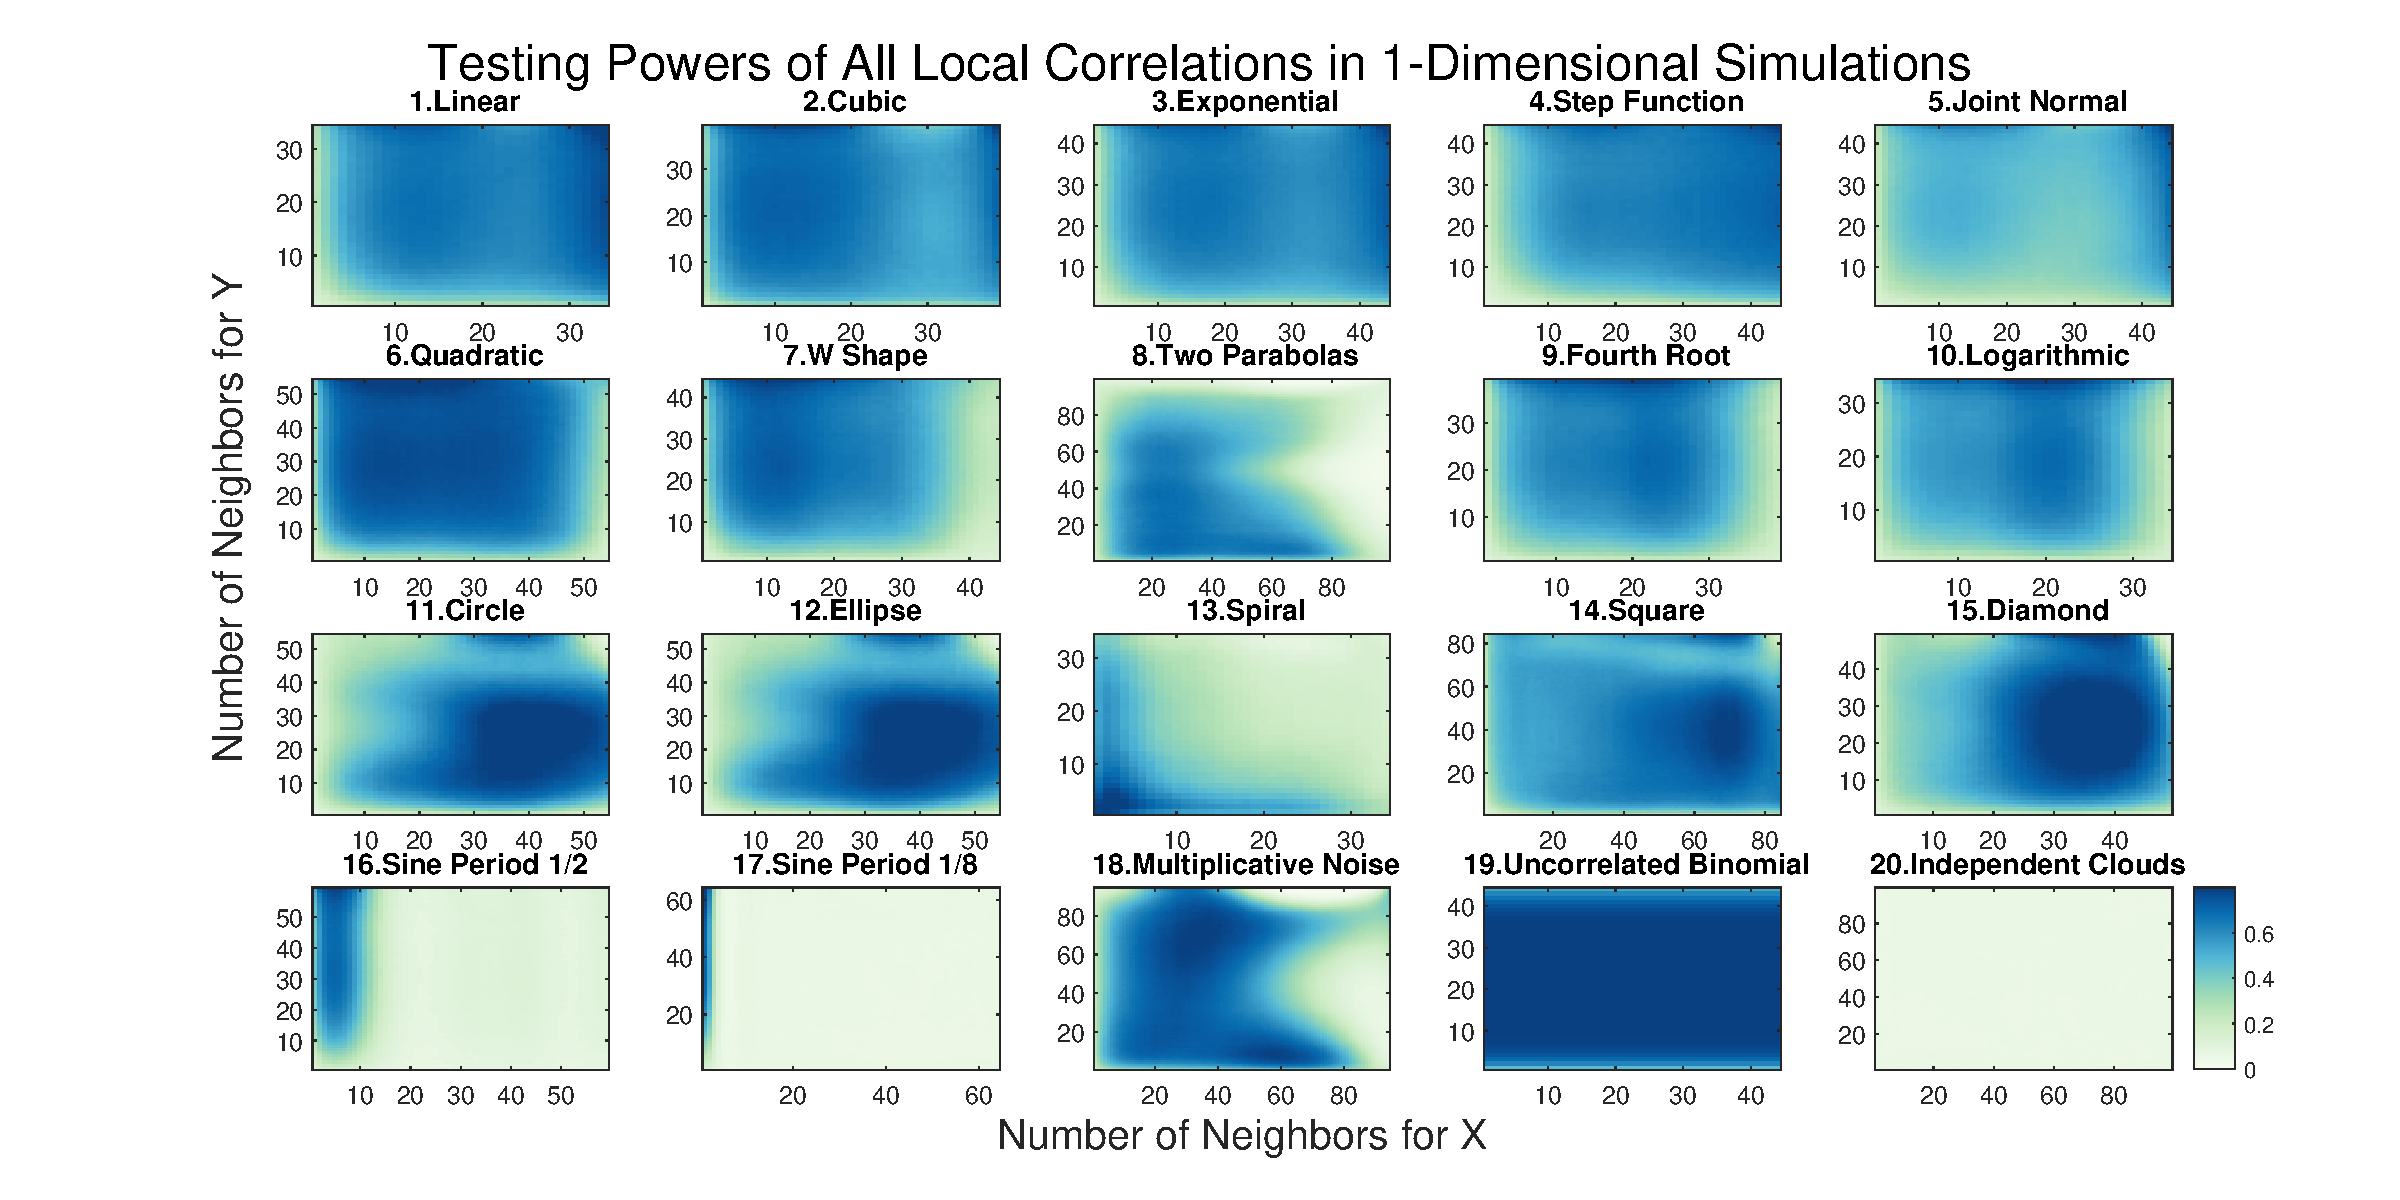
\includegraphics[width=1.0\textwidth]{../Figures/Fig2}
}
\hfil
\subfloat[]{
\includegraphics[width=1.0\textwidth]{../Figures/Fig6}
}
\caption{Testing Power for 20 Simulations with respect to Increasing Neighborhoods}
\label{figSim2}
\end{figure}

\begin{figure}[htbp]
\subfloat[]{
\includegraphics[width=0.5\textwidth]{../Figures/Fig4}
}
\hfil
\subfloat[]{
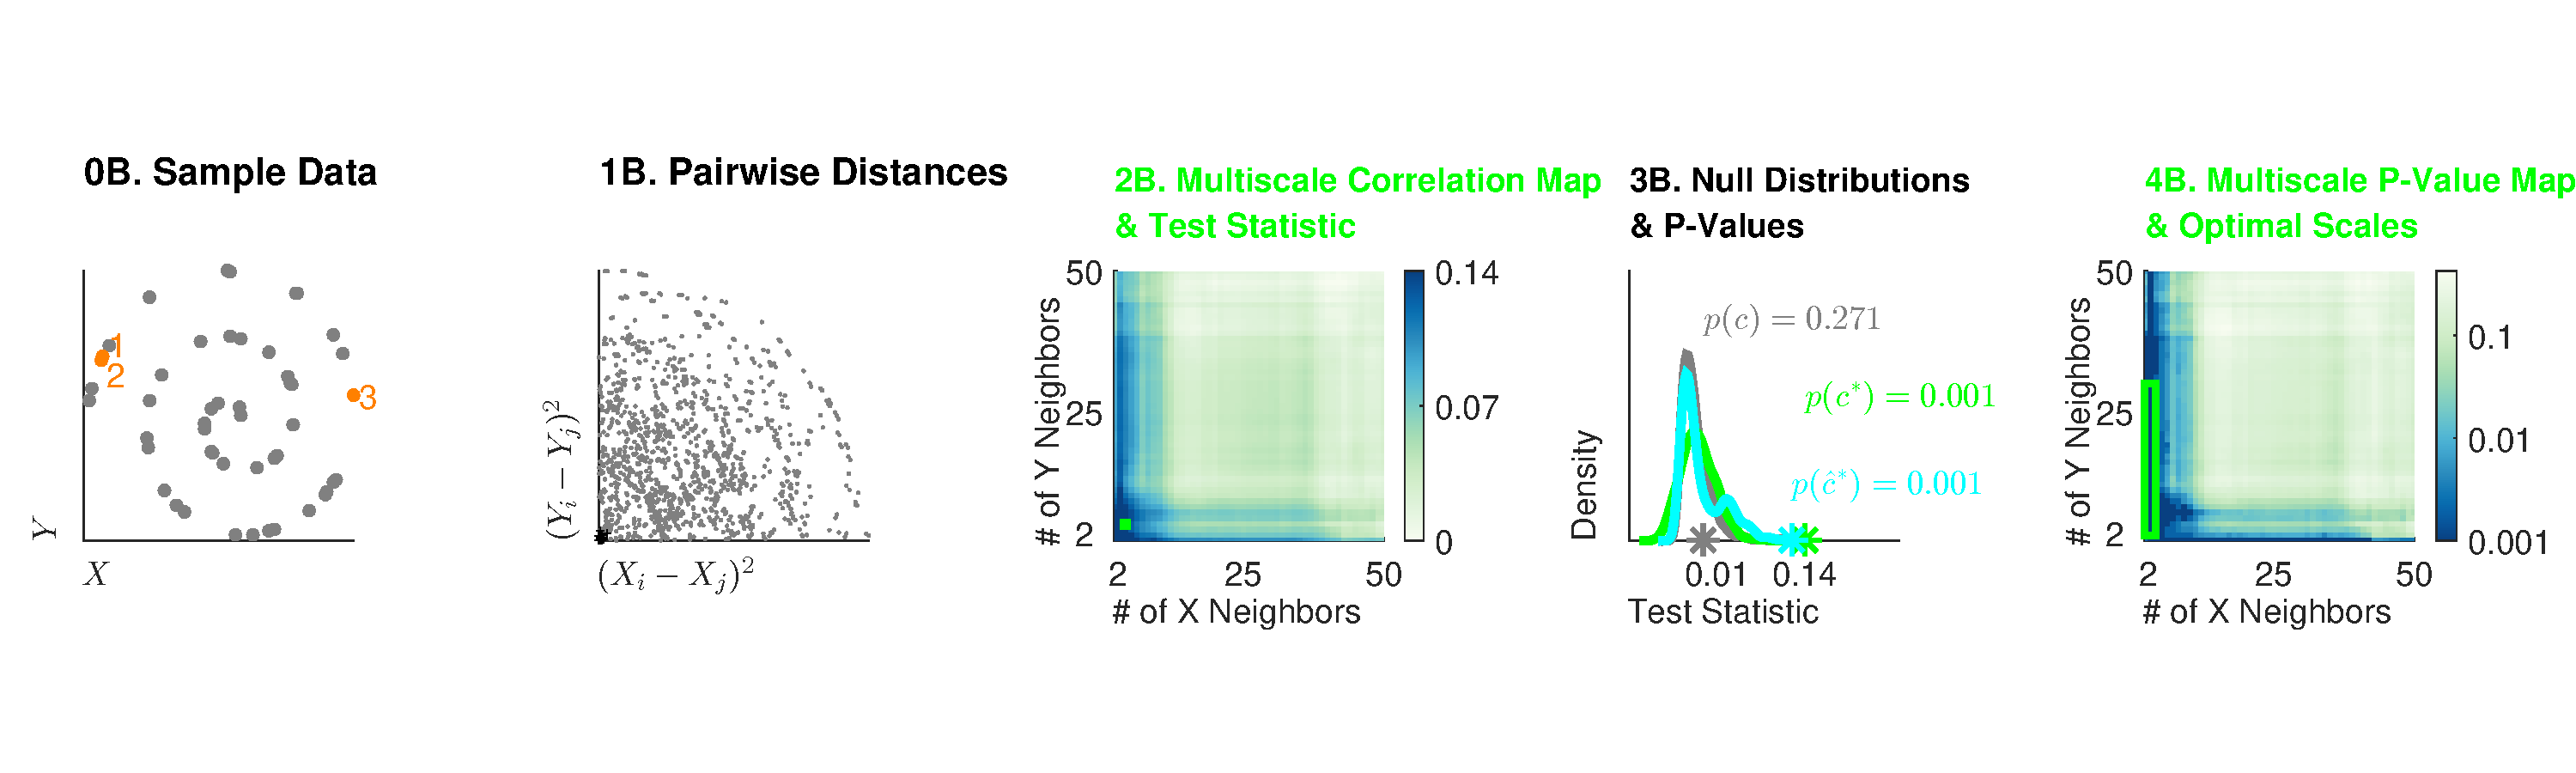
\includegraphics[width=0.5\textwidth]{../Figures/Fig8}
}
\caption{Area under Curve of Performance Profiles for 20 Simulations}
\label{figSim4}
\end{figure}


\bibliographystyle{chicago}
\bibliography{references}

\end{document}